%
% $Id: ch03_thework.tex
%
%   *******************************************************************
%   * SEE THE MAIN FILE "AllegThesis.tex" FOR MORE INFORMATION.       *
%   *******************************************************************
%
\chapter{Method of Approach} \label{ch:methods}

\name\ was developed using a modified agile approach; short development ``sprints'' were executed for key system development.
We describe the product of some of those sprints in Section~\ref{ch:methods:renderer}, primarily the ray-tracing engines.
In Section~\ref{ch:methods:interface} we also describe the Tickit interface and its algorithms.
Finally, in Section~\ref{ch:methods:threats}, we discuss drawbacks, challenges, and failures in development, as well as directions for future improvement as an open source project.


\section{Renderer Implementation} \label{ch:methods:renderer}
While building \name, two separate render engine prototypes were implemented.
The first, which we describe in Section~\ref{ch:methods:renderer:sequential}, was a simple, single core sequential renderer \cite{raytermCpuImpl}.
This engine was developed in three main development sprints, over a period of about two months.
The second, described in Section~\ref{ch:methods:renderer:parallel}, uses CUDA \cite{nvidia2011cuda} and OptiX \cite{parker2010optix} to leverage GPU compute power in parallel.
This engine was developed over two sprints, in a little under a month.


\subsection{Sequential} \label{ch:methods:renderer:sequential}

The sequential renderer, or \texttt{rayterm-cpu}, is a CPU-only ray-tracer.
It supports three different types of materials: diffuse, metallic, and dielectric.
These materials are complemented with two geometric primitives: disks, and spheres.
Figure~\ref{fig:rayterm-cpu_ppm} shows an image of the \texttt{ppm} output of \texttt{rayterm-cpu} near the end of its development.
The Tickit interface was never integrated into the CPU implementation, as this implementation is not performant enough for even simple scenes at low resolution.
For example, Figure~\ref{fig:rayterm-cpu_ppm} was rendered in about twenty seconds on a modern CPU.

\vspace{0.3em}
\begin{figure}[htb]
  \centering
  \includegraphics[width=0.75\textwidth]{impl-images/first_positionable_camera}
  \caption{\texttt{rayterm-cpu} example \texttt{ppm} output}
  \label{fig:rayterm-cpu_ppm}
\end{figure}

The main advantage of a sequential renderer is the lower development overhead, since there is no need to interface with a complex device such as a GPU.
This means that there is no need for handling parallel execution, and each ray is computed one after the other.
Because of this simplicity, this engine's development was perfectly suited for the goal of gaining knowledge and experience in ray-tracing.
The development also explored many fundamentals so that future contributions would be well-founded.
With 219 commits and over a thousand lines of code in the final product, along with many thousands of additions and deletions, \texttt{rayterm-cpu} accomplished its goals.

\littlesection{Components} \label{ch:methods:renderer:sequential:components}

The sequential renderer's implementation relies on two main components, as well as the Eigen linear algebra library \cite{eigenweb}.
These components have a linear relationship, as can be seen in Figure~\ref{fig:rayterm-cpu_components}; \texttt{raytrace} deals with tracing rays, \texttt{raymath} with intersection logic, and Eigen with linear algebra.

\vspace{0.3em}
\begin{figure}[htb]
  \centering
  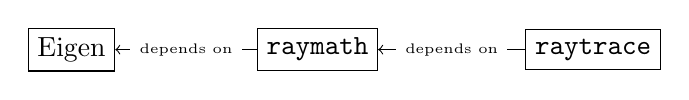
\begin{tikzpicture}
      \node[shape=rectangle,draw=black] (e) at (-3.125,0) {Eigen};
      \node[shape=rectangle,draw=black] (rm) at (0,0) {\texttt{raymath}};
      \node[shape=rectangle,draw=black] (rt) at (3.5,0) {\texttt{raytrace}};

      \path [<-](e) edge node[midway, fill=white] {\tiny depends on} (rm);
      \path [<-](rm) edge node[midway, fill=white] {\tiny depends on} (rt);
  \end{tikzpicture}
  \caption{Component and dependency relationships in \texttt{rayterm-cpu}}
  \label{fig:rayterm-cpu_components}
\end{figure}

Eigen \cite{eigenweb} is a linear algebra for C++ that supports matrix and vector manupulations, various matrix decompositions and geometry features, and has many extensions for numerous other numerical operations.
Eigen is also extremely well-optimized and uses SSE vectorized code, vastly improving performance on supported CPUs.
In \texttt{raymath}, Eigen is used primarily for easy, tested representations and calculations involving vectors; all of the algorithms implemented use equations derived from the ones in Section~\ref{ch:intro:background:raytracing_math}, and so benefit from easy implementation.

The base component in \texttt{rayterm-cpu} -- \texttt{raymath} -- provides support for various geometries and intersection routines. The geometries supported can be seen in Figure~\ref{fig:rayterm-cpu_raymath_geometry}, and use Eigen structures to represent their geometric data.
\texttt{raymath} also handles random number and vector generation, color handling, and intersection representation.
The implementations behind these are covered in Section~\ref{ch:implementation:rayterm-cpu:raymath}.

\vspace{0.3em}
\begin{figure}[htb]
  \centering
  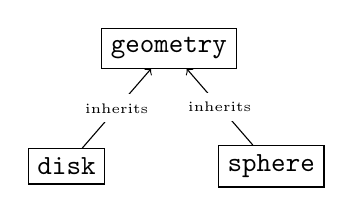
\begin{tikzpicture}
    \node[shape=rectangle,draw=black] (g) at (0,1.5) {\texttt{geometry}};
      \node[shape=rectangle,draw=black] (s) at (1.3,0) {\texttt{sphere}};
      \node[shape=rectangle,draw=black] (d) at (-1.3,0) {\texttt{disk}};

      \path [<-](g) edge node[midway, fill=white] {\tiny inherits} (s);
      \path [<-](g) edge node[midway, fill=white] {\tiny inherits} (d);
  \end{tikzpicture}
  \caption{Geometric structures in \texttt{raymath}}
  \label{fig:rayterm-cpu_raymath_geometry}
\end{figure}

The main component in \texttt{rayterm-cpu} is \texttt{raytrace}; it handles world representation, materials, and raytracing.
\texttt{rayterm-cpu} only renders in \texttt{ppm} mode, since the Tickit interface was only integrated in the \texttt{rayterm-gpu} implementation, since that was the final prototype.
\texttt{raytrace} represents objects with a \texttt{WorldObject} class, a list of which is stored in a \texttt{World}.

Figure~\ref{fig:rayterm-cpu_raytrace_journey_of_a_ray} shows the function call path that is used when rendering a single ray.
The main entry point is \texttt{raytrace\_ppm}, which creates rays with a \texttt{Camera} class instance.
This instance contains specific parameters to control the position and orientation of the virtual camera, and thus controls where the \texttt{ray} originates from. and its direction.
Then, that \texttt{ray} is sent on to the \texttt{World} class, where an \texttt{intersection} is retrieved, and then used to generate a \texttt{color} from the given \texttt{ray}.
This color is then finally returned to \texttt{raytrace\_ppm}, which writes it to a \texttt{ppm} file.
Unmentioned in this diagram are the recursive calls to \texttt{World::trace} from from \texttt{WorldObject::colorize}, which use the transformed ``scatter'' \texttt{ray} from \texttt{Material::scatter}.
The implementation behind all of these structures and functions are covered in Section~\ref{ch:implementation:rayterm-cpu:raytrace}.

\vspace{0.3em}
\begin{figure}[htb]
  \centering
  \begin{tikzpicture}
    \node[shape=rectangle, draw=black] (a) at (0,0) {Ray collection in \texttt{raytrace\_ppm}};
    \node[shape=rectangle, draw=black, right = 2.5em of a ] (b) {Generation in \texttt{Camera::get\_screen\_ray}};
    \node[shape=rectangle, draw=black, below = 1.75em of a] (c) {World tracing in \texttt{World::trace}};
    \node[shape=rectangle, draw=black, right = 2.5em of c] (e) {Ray coloring in \texttt{WorldObject::colorize}};
    \node[shape=rectangle, draw=black, below = 1.75em of e] (s) {Ray scattering in \texttt{Material::scatter}};
    \node[shape=rectangle, draw=black, below = 1.75em of c] (d) {World intersection in \texttt{World::intersects}};
    \begin{scope}[xshift=1cm]
      \node[shape=rectangle, draw=black] (f) at (2.75, -4.15) {Object intersection in \texttt{WorldObject::intersects}};
      \node[shape=rectangle, draw=black, below = 1.75em of f] (g) {Geometry intersection in \texttt{geometry::intersects}};
      \path [->](d) edge node[midway, fill=white] {\tiny calls} (f);
      \path [->](f) edge node[midway, fill=white] {\tiny calls} (g);
    \end{scope}

      \path [->](a) edge node[midway, fill=white] {\tiny calls} (b);
      \path [->](a) edge node[midway, fill=white] {\tiny calls} (c);
      \path [->](c) edge node[midway, fill=white] {\tiny calls} (d);
      \path [->](c) edge node[midway, fill=white] {\tiny calls} (e);
      \path [->](e) edge node[midway, fill=white] {\tiny calls} (s);
  \end{tikzpicture}
  \caption{The journey of a \texttt{ray} and its \texttt{intersection}}
  \label{fig:rayterm-cpu_raytrace_journey_of_a_ray}
\end{figure}

\littlesection{Algorithms} \label{ch:methods:renderer:sequential:algorithms}

The sequential renderer implements single-branch Monte Carlo ray-tracing, a type of rendering that can produce physically accurate images with little development effort.
The algorithm is largely based on randomness, only modifying the path of a single ray at a time as it bounces around the scene.
When encountering objects, a particular Probability Distribution Function (PDF) is used to calculate where the ray will bounce.
These PDFs vary based on the material, and are hardcoded in the \texttt{Material} implementation.
The result of this algorithm is extremely noisy because of this randomness (see Figure~\ref{fig:rayterm-cpu_ppm_noisy}), so many samples must be taken and then averaged to gain a true value for a single pixel; this simulates the many millions of photons that would have traveled to that pixel in a real camera.
The number of samples per pixel, sometimes termed ``spp,'' is the number of rays generated from a random origin within the pixel; this is done for every pixel in the image.
An example of various spp values is shown in Figure~\ref{fig:rayterm-cpu_ppm_noisy}.

\vspace{0.3em}
\begin{figure}[htb]
  \centering
  \begin{subfigure}[htb]{0.45\textwidth}
    \includegraphics[width=\textwidth]{impl-images/comparisons/samples_spp_1}
    \caption{1 sample per pixel}
    \label{fig:rayterm-cpu_ppm_noisy_1}
  \end{subfigure}
  \hspace{1em}
  \begin{subfigure}[htb]{0.45\textwidth}
    \includegraphics[width=\textwidth]{impl-images/comparisons/samples_spp_4}
    \caption{4 samples per pixel}
    \label{fig:rayterm-cpu_ppm_noisy_4}
  \end{subfigure}
  \vspace{1em}
  \begin{subfigure}[htb]{0.45\textwidth}
    \includegraphics[width=\textwidth]{impl-images/comparisons/samples_spp_32}
    \caption{32 samples per pixel}
    \label{fig:rayterm-cpu_ppm_noisy_32}
  \end{subfigure}
  \hspace{1em}
  \begin{subfigure}[htb]{0.45\textwidth}
    \includegraphics[width=\textwidth]{impl-images/comparisons/samples_spp_1024}
    \caption{1024 samples per pixel}
    \label{fig:rayterm-cpu_ppm_noisy_1024}
  \end{subfigure}
  \caption{Sample per pixel differentiated output from \texttt{rayterm-cpu}}
  \label{fig:rayterm-cpu_ppm_noisy}
\end{figure}

For an spp value of four, there are four rays generated for each pixel; thus, the rendering equation \cite{kajiya1986rendering} is approximated at the first intersection by four random direction samplings (keep in mind the integration is over the sphere or hemisphere around the point of intersection for each ray).
Thus, the more rays generated, the more accurate that sampling becomes.
This is still not really solving the rendering equation, and is a large simplification.
Rather, the different eye-rays generated because of the spp value sample slightly different intersection points.
These rays then also sample different directions out of those intersection points, and so are a kind of ``fuzzy'' approximation.
An area for future work is implementing a kind of ``stratification'' of these samples, so that they are not randomly spread, but instead fully sample the sphere or hemisphere at a certain resolution;
This would likely be combined with branched Monte Carlo rendering, which involves generating multiple rays for each intersection hit, thereby actually sampling the same integral.
This would reduce the noise at low spp values significantly better than simply increasing the spp value, although at the slight cost of performance (more rays to calculate).

\begin{equation}
  \label{equation:raytracing_ops}
  N_{ops} = R \cdot S \cdot D \cdot N
\end{equation}

In discussing the complexity of this implementation, there are four main variables to keep in mind: first, the number of pixels to render, $R$; second, the number of samples per pixel, $S$; third, the maximum number of recursions per sample, $D$; and fourth, the number of intersectable objects in the scene, $N$.
The number of pixels to render varies with the resolution of the desired image.
The number of samples per pixel and the maximum number of recursions are both user-specified configurable values.
The number of objects in the scene can vary wildly, but most test scenes in \texttt{rayterm-cpu} have less than $10$ objects.
This gives us Formula~\ref{equation:raytracing_ops} to calculate the number of base ``ray tracing operations,'' which we call $N_{ops}$.
These operations consist of a single ray-tracing intersection operation, which involves testing a ray against a single parametric equation for intersection.
As long as that operation can be considered constant, $O(R \cdot S \cdot D \cdot N)$ is the time complexity of the Monte Carlo algorithm used in \texttt{rayterm-cpu}.
For spheres and disks, the only geometry supported, the intersection routine depends on both $sqrt()$ and $dot()$.
However, the time complexities of these functions probably do not vary with respect to the value given to them.
For taking the square root, there is likely system support for fast calculation independent of input value; for vector dot products, the size is always constant at three entries.
Because of this, we can consider the time complexity of a single intersection test to be constant.
Thus, the time to complete a render varies proportional to the number of objects in the scene, the resolution of the image, the number of samples per pixel, and the ray-tracing depth.

As an example, take a scene with $3$ spheres and a disk.
Let us render an $80$ by $52$ pixel image;
we will choose to use $32$ samples per pixel to get a reasonable image quality.
For maximum recursion depth a value of $5$ should be plenty for the simple scene we have -- a more complex scene could probably benefit from a few more, but since attenuation reduces the impact each successive ray has on a fragment, it is very unlikely to matter past a few tens.
Thus, we have all the information we need: $R = 4160,\ S = 32,\ D = 5,\ N = 4$.
We can calculate the final number of basic ray-tracing intersections by simply multiplying these variables together: we get $2662400$.
Since this kind of image can usually be rendered in around 200 milliseconds by \texttt{rayterm-cpu}, we can get a sense of how fast the existing intersection is already: one test takes about $75$ nanoseconds.
There's not much hope of drastically improving this time.
Even to get render time down to $33$ milliseconds, which is needed for a $30$ frame per second playback, we would need an intersection test to take no more than $12.4$ nanoseconds.
This is nigh impossible with modern CPUs -- for comparison, basic multiplication takes an average 19 nanoseconds on an i7-4770k, a relatively modern processor -- the code to calculate this value on any computer can be seen in Appendix~\ref{appendix:timemul}.

Therefore any further major performance improvement needs to break out of the sequential world this algorithm was written in.

The algorithms used for intersection are already covered in Section~\ref{ch:intro:background:raytracing_math}; however the scattering algorithms are discussed here.
There are three materials supported in \texttt{rayterm-cpu}: Lambertian, metallic, and dielectric.
The Lambertian material, sometimes known as diffuse, is very simple; the scattered ray originates at the intersection location, and the direction is random in the unit hemisphere oriented about the surface normal of the intersected object.
Essentially, when a ray hits a Lambertian object the ray reflects around the tiny crevices and cracks on the surface of the object so that the direction is entirely random once it leaves the object.

\begin{equation}
  \label{equation:reflection}
  \vec{R_{reflect}} = \vec{R_{in}} - 2(\vec{S_{normal}} \bullet \vec{R_{in}})\vec{S_{normal}}
\end{equation}

The metallic material scatters rays in a similar way as the Lambertian, but includes a bias towards the reflection direction.
The reflection direction is calculated using Formula~\ref{equation:reflection} \cite{prunier2017shading}, where $\vec{R_{reflect}}$ is the reflected ray, $\vec{R_{in}}$ is the incoming ray, and $\vec{S_{normal}}$ is the surface normal.
The bias is generated by using a ray direction that is linearly interpolated between the pure reflection direction from Formula~\ref{equation:reflection} and a random direction generated as in Lambertian materials.
The amount of linear interpolation is known as the ``roughness'' -- a roughness of zero gives perfect reflection (a mirror), whereas a roughness of one gives the same results as a Lambertian material.
A slightly more accurate roughness ramp could be attained by using spherical linear interpolation, however because of the significant performance penalty that was not used.

Finally, the dielectric material is the most complicated.
A dielectric material supports both reflection (as in the other materials), and refraction.
Since we scatter only one ray at a time, the scatter function uses probability to determine which kind of trajectory will be used.
This probability is based on Schlick's approximation of the fresnel factor, as seen in Formula~\ref{equation:schlick} \cite{schlick1994inexpensive, learnopengltheory, prunier2017shading}.
In this approximation, $\theta$ is the angle between the incoming ray direction and the surface normal; $n_1$ and $n_2$ are the indices of refraction of the object and air -- these are reversed if the ray is leaving the object.
Finally, $R_0$ is the value of the Fresnel term when there is minimal reflection \textit{i.e.} when $\theta = 0$.

\begin{equation}
  \label{equation:schlick_base}
  R_0 = (\frac{n_1 - n_2}{n_1 + n_2})^2
\end{equation}
\begin{equation}
  \label{equation:schlick}
  R(\theta) = R_0 + (1 - R_0)(1 - cos \theta)^5
\end{equation}

This approximation gives values close to $0$ when the view angle is high, for example when looking directly through an object; it gives values close to $1$ when the view angle is low, for example on the oblique sides of a sphere.
This can be seen in Figure~\ref{fig:rayterm-cpu_fresnel}: notice that the gradient is not linear and the white is mostly concentrated on the oblique edges of the sphere.
The approximation is then used to determine if the ray will be refracted (low values) or reflected (high values) by testing against a random scalar in the range $[0, 1)$.
This will result in high viewing angles (black in Figure~\ref{fig:rayterm-cpu_fresnel}) generating refraction rays, and low viewing angles (white in Figure~\ref{fig:rayterm-cpu_fresnel}) generating reflection rays.
This is a close approximation of the effect that glass and other dielectrics have when viewed in the real world.

\vspace{0.3em}
\begin{figure}[htb]
  \centering
  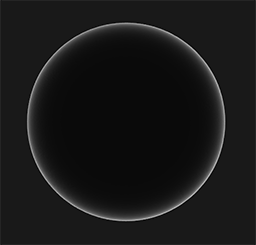
\includegraphics[width=0.4\textwidth]{resources/fresnel}
  \caption{Schlick approximation for a sphere (white is $1$, black is $0$) \cite{learnopengltheory}}
  \label{fig:rayterm-cpu_fresnel}
\end{figure}

Now that the kind of ray has been chosen, the refraction or reflection direction is calculated.
There is an additional possibility that the specific ray we have cannot be refracted because of total internal reflection -- in this case, we switch over to a reflection ray.
The ray direction in the reflection case is calculated with Formula~\ref{equation:reflection} as in previous materials.
The ray direction in the refraction case is calculated with Formula~\ref{equation:refraction}.
In this formula, $\vec{R_{refract}}$ is the refracted ray; $n_{from}$ is the index of refraction of the medium we are transfering from, and $n_{to}$ is the corresponding index; $\vec{R_{in}}$ is the incoming ray; and $\vec{S_{normal}}$ is the surface normal.
There is some additional handling in the implementation of this formula to ensure both ray directions (exiting and entering an object) are supported.
This involves flipping the $n$ values and negating $I$ or $\vec{S_{normal}}$.
This formula is derived from the excellent ``Scratchapixel'' \cite{prunier2017shading} and ``Raytracing in One Weekend'' \cite{shirley2016ray}, with some significant rewriting.
\begin{equation}
  \label{equation:refraction_eta}
  \eta = \frac{n_{from}}{n_{to}}
\end{equation}
\begin{equation}
  \label{equation:refraction_i}
  I = (\vec{R_{in}} \bullet \vec{S_{normal}})
\end{equation}
\begin{equation}
  \label{equation:refraction}
  \vec{R_{refract}} = \eta\vec{R_{in}} + (\eta I - \sqrt{1 - \eta^2 \cdot (1 - I^2)})\vec{S_{normal}}
\end{equation}

\littlesection{Prototype} \label{ch:methods:renderer:sequential:prototype}

This section describes the lessons learned from CPU implementation, and how the GPU implementation will differ and improve because of this step.

The final implementation of \texttt{rayterm-cpu} only renders images through a Google Test \cite{googletest} case, which can be run with the \texttt{test.sh} script in the implementation repository \cite{raytermCpuImpl}, or \texttt{gradle test}.
This generates a \texttt{test\_image.ppm} file, examples of which we show from various stages of development in Section~\ref{ch:implementation:rayterm-cpu:raytrace}.
Because of this, \texttt{rayterm-cpu} is very much a proof-of-concept and learning example, rather than a fully-fledged library.

\subsection{Parallel} \label{ch:methods:renderer:parallel}

After the implementation of \texttt{rayterm-cpu}, more performance was needed for the final \name\ implementation.
The solution to this problem was to use a Graphics Processing Unit (GPU) to drastically parallellize the raytracing algorithm.
This improves performance dramatically, because each eye-ray's children (the result of a collision between an object and a ray) are dependant on only their parent eye-ray.
Thus, the computation of a single pixel's color is completely independent of every other pixel.

A short introduction to GPUs may be useful here; they consist primarily of small units of computation circuitry called ``multiprocessors'' which themselves are controllers for several CUDA cores \cite{fermi2009nvidia}, distributing workloads.
These CUDA cores execute individual threads on the GPU, and act somewhat like advanced floating point arithmatic computation units.
A discussion on the specific hardware used for development and testing is available in Section~\ref{ch:intro:background:hardware}.

With 227 commits and over 1.5 thousand lines of code, along with many thousands of additions and deletions, \texttt{rayterm-gpu} has a good start on its life.
There are many, many more improvements possible, however.
We detail some of them in the context of the larger \name\ implementation in Section~\ref{ch:methods:threats}.

\littlesection{Libraries} \label{ch:methods:renderer:parallel:libraries}

This section talks about OptiX and CUDA.

\littlesection{Design} \label{ch:methods:renderer:parallel:design}

This section is about the code structure and organization in the \texttt{rayterm} implementation.

\littlesection{Demonstration} \label{ch:methods:renderer:parallel:demo}

This is a demonstration section on final renderer is capabable of -- this section uses only \texttt{ppm} output.

\section{Interface Implementation} \label{ch:methods:interface}

\subsection{Design} \label{ch:methods:interface:design}
